\capitulo{Procedimentos metodológicos e técnicos}
\label{cap:procedimentos-metodologicos-tecnicos}

Neste capítulo do trabalho será abordada a caracterização da metodologia de pesquisa, questões de pesquisa,
como será a aplicação da metodologia e o planejamento do desenvolvimento da integração com Alexa, além de mostrar como será planejada a análise de resultados e a população e amostra do trabalho.

\secao{Caracterização da metodologia de pesquisa}
\label{sec:caracterizacao-metodologia-pesquisa}
    
A metodologia escolhida para o planejamento do desenvolvimento da integração entre Amazon Alexa e o aplicativo Pollen é a Metodologia em Cascata, 
proposta por \textcite{sommerville2011} e amplamente utilizada em projetos de desenvolvimento de software.

A Metodologia em Cascata é um modelo de desenvolvimento de software que divide o processo em etapas sequenciais e bem definidas, 
garantindo que cada fase seja concluída antes de avançar para a próxima. Essa abordagem permite um controle mais rigoroso sobre o progresso do projeto e facilita a identificação e correção de possíveis problemas ao longo do planejamento.

Os procedimentos técnicos adotados neste trabalho envolvem a realização de uma \textbf{pesquisa bibliográfica}, de um \textbf{estudo de caso} e o \textbf{planejamento de uma pesquisa experimental}.

A pesquisa bibliográfica fornece o embasamento teórico necessário para a definição dos padrões de desenvolvimento de Alexa Skills e integração com APIs, essenciais para o planejamento da solução.

O estudo de caso consiste na análise do aplicativo Pollen e identificação das funcionalidades que podem ser integradas com assistentes virtuais, permitindo uma análise aprofundada das possibilidades de integração. O enfoque será direcionado para apicultores usuários do aplicativo Pollen, o que delimita o escopo da pesquisa.

O planejamento da pesquisa experimental será conduzido mediante a definição de metodologias para desenvolvimento e teste da integração Alexa+Pollen com apicultores reais, que utilizarão a skill planejada em seus ambientes de trabalho. O objetivo é planejar a avaliação da eficácia da solução em contextos reais de gestão apícola.
    
    
\secao{Questões de Pesquisa}
\label{sec:questoes-pesquisa}

A integração proposta entre Amazon Alexa e o aplicativo Pollen é capaz de fornecer acesso eficiente 
a informações sobre colmeias através de comandos de voz, melhorando a experiência do usuário 
e facilitando o trabalho no apiário sem necessidade de interromper as atividades para consultar dispositivos móveis?

\secao{Aplicação da metodologia}
\label{sec:aplicacao-metodologia}

Nesta subseção, são descritas as etapas planejadas para a metodologia deste trabalho. As atividades englobam desde o planejamento do ambiente de desenvolvimento e coleta de requisitos até o 
planejamento da implementação da integração Alexa+Pollen e a validação dos resultados obtidos. Cada fase será planejada com o objetivo de garantir a confiabilidade do planejamento do sistema e a coerência com os objetivos traçados neste trabalho.

\subsecao{Planejamento do desenvolvimento da solução proposta}
\label{ssec:planejamento-desenvolvimento-solucao}

O modelo em cascata é uma das abordagens clássicas para o desenvolvimento de software e foi originalmente descrito por Winston Royce em 1970. 
Este modelo foi posteriormente estruturado por Ian Sommerville em sua obra clássica “Engenharia de Software” como um processo sequencial em que cada fase depende da entrega da anterior e gera um produto definido.

\begin{figura}{Modelo Cascata}{\textcite{sommerville2011}}
    \begin{flushleft}
        \label{fig:modelo-cascata}
        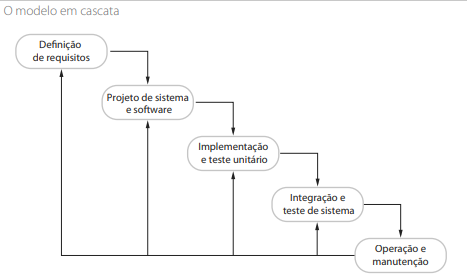
\includegraphics[width=0.95\linewidth]{resources/floats/ilustracoes/cascata.png}
    \end{flushleft}
\end{figura}

Conforme ilustrado na Figura \ref{fig:modelo-cascata} (Modelo cascata de Sommerville), o modelo é dividido em cinco fases principais: definição de requisitos, 
projeto de sistema e software, implementação e teste unitário, integração e teste de sistema, e operação e manutenção. 
Cada fase possui entregáveis específicos e critérios de entrada e saída bem definidos.

\subsubsecao{Definição de Requisitos}
\label{sssec:def-requisitos}

A definição de requisitos é a etapa de desenvolvimento de software que descreve detalhadamente o que o sistema deve fazer e quais restrições ele deve obedecer. 
De acordo com \textcite{sommerville2011}, um requisito é "uma descrição de algo que o sistema deve fazer ou uma propriedade que ele deve ter" \cite[p. 82]{sommerville2011}. 
Essa definição engloba tanto funcionalidades esperadas quanto limitações técnicas ou organizacionais que devem ser consideradas na construção do projeto.

Ainda segundo \textcite{sommerville2011}, os requisitos funcionais especificam os serviços que o sistema deve oferecer e como ele deve reagir a entradas específicas. 
Por outro lado, os requisitos não funcionais dizem respeito a restrições sobre os serviços ou funções oferecidas, como requisitos de desempenho, padrões de qualidade, requisitos organizacionais ou de segurança. 
Para a obtenção desses requisitos, será adotada a técnica de entrevistas semiestruturadas com os usuários finais que serão apicultores usuários do aplicativo Pollen. 
Essa abordagem permitirá captar informações sobre as necessidades práticas dos usuários, possibilitando uma definição mais precisa e contextualizada dos requisitos do sistema.

\subsubsecao{Projeto de Sistema e Software}
\label{sssec:proj-sistema}

A fase de projeto de sistema e software visa transformar os requisitos previamente definidos em uma arquitetura viável para implementação. 
De acordo com \textcite{sommerville2011}, o projeto de software é o processo de definir a arquitetura, os componentes e suas interfaces, garantindo que o sistema satisfaça os requisitos especificados. 
Neste projeto, essa etapa se desdobra em três frentes principais: Desenvolver uma Alexa Skill personalizada, integrar com o aplicativo Pollen e testar a integração com usuários reais.

O desenvolvimento da Alexa Skill personalizada será feito utilizando o Amazon Alexa Skills Kit e Node.js seguindo as melhores práticas de desenvolvimento de Alexa Skills. O processo de criação envolve o registro da skill no Amazon Developer Console, configuração do modelo de interação e desenvolvimento do backend utilizando AWS Lambda.

A integração com o aplicativo Pollen será realizada através de chamadas HTTP para a API RESTful existente, utilizando autenticação JWT seguindo as melhores práticas de segurança. 

A testagem da integração será feita com usuários reais utilizando o aplicativo Pollen e a Alexa Skill desenvolvida.

As Figuras \ref{fig:criacao-skill}, \ref{fig:linguagens-skill} e \ref{fig:teste-skill} ilustram as principais etapas do processo de desenvolvimento no Amazon Developer Console. A Figura \ref{fig:criacao-skill} exemplifica a interface de criação de uma nova Alexa Skill, onde são configurados o nome da skill, o idioma de suporte e as informações básicas do projeto. A Figura \ref{fig:linguagens-skill} demonstra as opções de idiomas disponíveis, sendo que a Skill será desenvolvida em português brasileiro, garantindo uma experiência natural para os usuários brasileiros do aplicativo Pollen. A Figura \ref{fig:teste-skill} apresenta a interface de teste da Skill, ferramenta essencial para simular comandos de voz e verificar se as respostas estão sendo geradas corretamente durante o desenvolvimento e antes da publicação.

A skill permitirá consultas sobre informações como número de colmeias, produção de mel, status dos enxames, próximas atividades de manejo e estatísticas de produtividade.

A implementação seguirá as melhores práticas de desenvolvimento de Alexa Skills, incluindo o uso de intents bem definidos, utterances em português brasileiro e respostas em formato SSML para melhor experiência do usuário.

\begin{figura}{Tela de criação de Skill Alexa}{O Autor}
    \begin{flushleft}
        \label{fig:criacao-skill}
        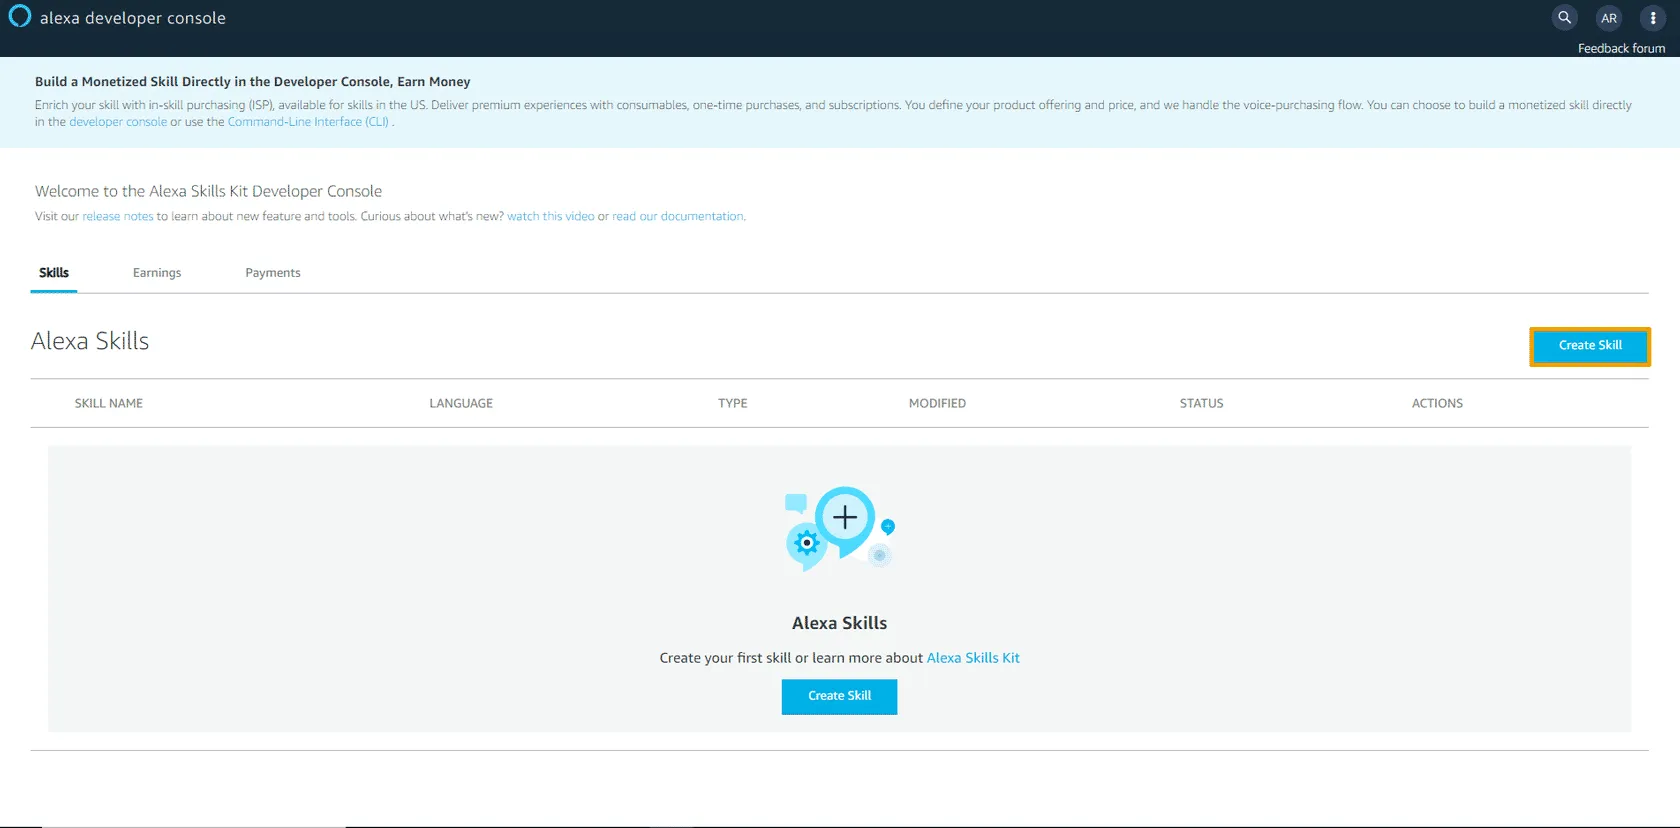
\includegraphics[width=0.85\linewidth]{resources/floats/ilustracoes/tela_criacao_skill_alexa.png}
    \end{flushleft}
\end{figura}

\begin{figura}{Tipos de linguagem aceitas pela Skill}{O Autor}
    \begin{flushleft}
        \label{fig:linguagens-skill}
        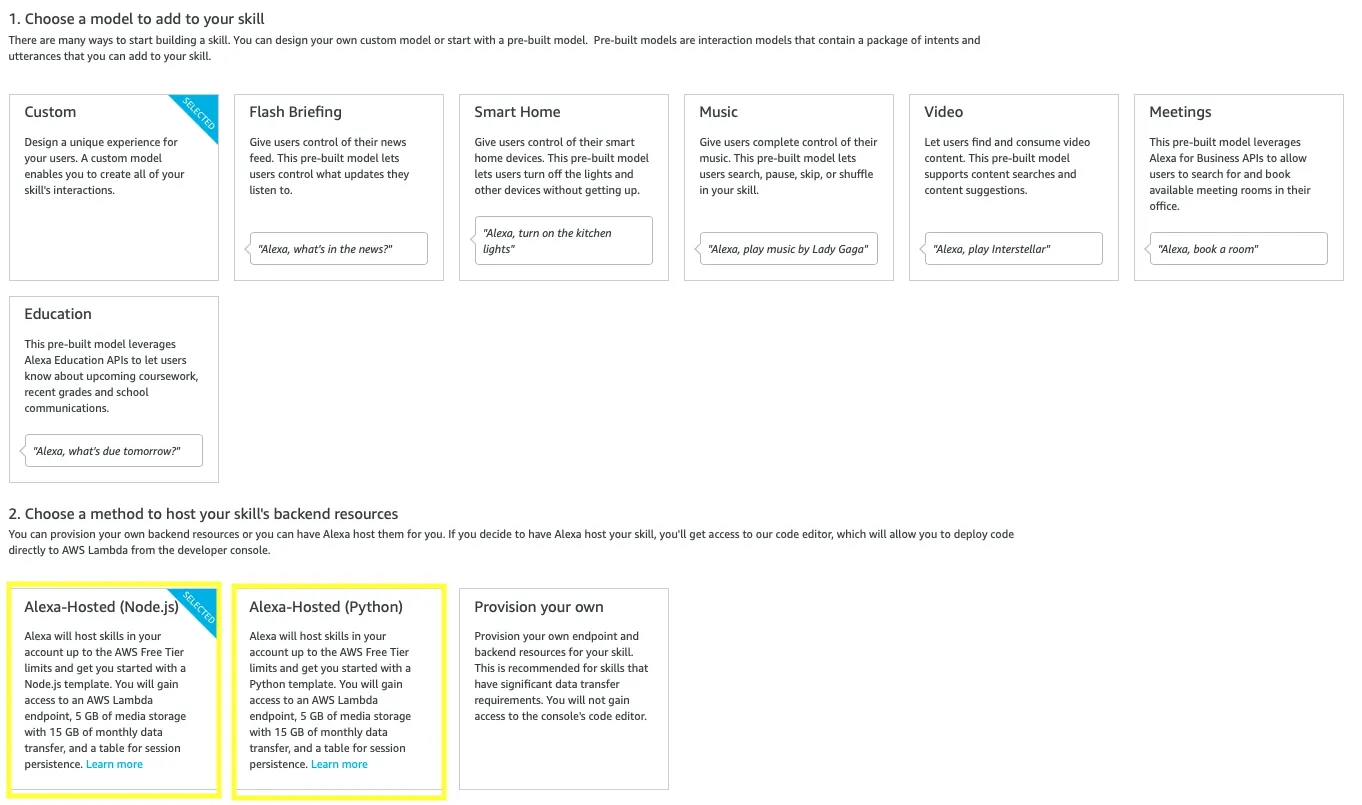
\includegraphics[width=0.85\linewidth]{resources/floats/ilustracoes/tipos_linguagem_aceitas_skill.png}
    \end{flushleft}
\end{figura}

\begin{figura}{Interface de teste da Skill Alexa}{O Autor}
    \begin{flushleft}
        \label{fig:teste-skill}
        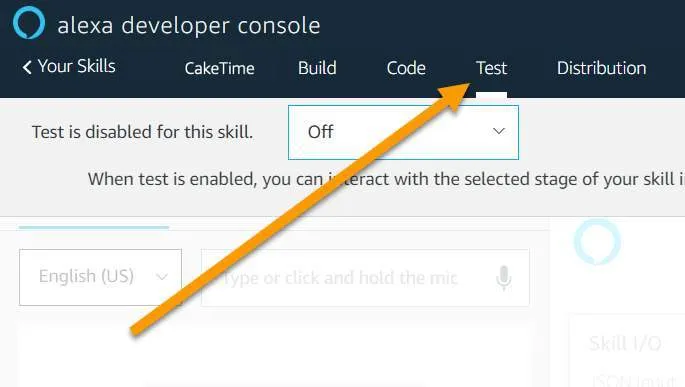
\includegraphics[width=0.85\linewidth]{resources/floats/ilustracoes/tela_para_testar_skill_criada.png}
    \end{flushleft}
\end{figura}

\subsubsecao{Fase de Implementação}
\label{sssec:implementação}


A fase de implementação representa o momento em que as decisões definidas nas etapas de projeto e análise se concretizam na construção prática do sistema. 
Segundo \textcite{sommerville2011}, essa etapa está diretamente relacionada à transformação dos modelos em código executável, respeitando os padrões estabelecidos e validando o funcionamento do sistema como um todo. 

O desenvolvimento da Alexa Skill será realizado utilizando Node.js e o Amazon Alexa Skills Kit (ASK). 
A skill será hospedada como uma função AWS Lambda, garantindo escalabilidade e confiabilidade no processamento das requisições. 
A comunicação com a API do aplicativo Pollen será implementada utilizando bibliotecas HTTP nativas do Node.js, com tratamento adequado de erros e timeouts.

A linguagem de programação escolhida para o desenvolvimento é Node.js com TypeScript. 
Serão utilizadas as bibliotecas oficiais do Alexa Skills Kit, além de bibliotecas para comunicação HTTP e processamento de dados JSON. 
A programação será conduzida na IDE VS Code, que permite integração com ferramentas de versionamento e ambientes virtuais.

O repositório da aplicação será controlado via Git e hospedado no GitHub, garantindo controle de versão, rastreabilidade de mudanças e backup do progresso. 
Isso também permitirá a integração com pipelines de entrega contínua futuramente, caso a aplicação seja expandida.

\subsubsecao{Tecnologias Utilizadas}
\label{sssec:tecnologias}

O desenvolvimento utilizará \textbf{Node.js com TypeScript} para implementação da Skill, devido ao suporte oficial da Amazon através do Alexa Skills Kit. A Skill será hospedada em \textbf{AWS Lambda}, garantindo escalabilidade e disponibilidade. A comunicação com o aplicativo Pollen ocorrerá via \textbf{API RESTful} já existente, utilizando autenticação \textbf{JWT} e protocolo \textbf{HTTPS} para segurança. O banco de dados \textbf{PostgreSQL} do Pollen será acessado indiretamente através da API, mantendo a arquitetura de camadas do sistema.

\subsubsecao{Fase de integração e testes}
\label{sssec:testes}

A fase de planejamento dos testes é responsável por planejar a garantia da qualidade do software e a conformidade com os requisitos especificados. 
Segundo \textcite{pressman2011}, os testes de software devem ser planejados de forma sistemática e aplicados com o propósito de revelar o maior número possível de defeitos, contribuindo para a qualidade e confiabilidade do produto final.

O planejamento dos testes será dividido entre a verificação funcional da Alexa Skill e a avaliação da integração com a API do Pollen. 
O roteiro de testes planejado considera a execução da skill com comandos de voz reais, testados por apicultores usuários do aplicativo Pollen. 
O objetivo é planejar a validação se as consultas por voz funcionam corretamente, se os dados retornados estão de acordo com os critérios esperados e se a experiência de uso da skill permanece fluida. 
As verificações funcionais planejadas incluem o reconhecimento correto dos comandos de voz, a comunicação adequada com a API do Pollen, a formatação apropriada das respostas em SSML, 
além da geração de respostas coerentes e do bom desempenho geral do sistema. Parte dos testes será também planejada para ser automatizada com o uso do framework Jest, 
focando em funções auxiliares como o processamento de intents e a validação da integração com a API, o que permite assegurar a estabilidade do sistema mesmo após possíveis futuras alterações no código.

Os testes serão realizados com apicultores usuários do Pollen, abrangendo testes unitários (processamento de intents e validação de dados), testes de integração (comunicação com API Pollen) e testes de aceitação do usuário (comandos de voz reais). Os critérios de sucesso incluem precisão de reconhecimento mínima de 90\%, tempo de resposta máximo de 3 segundos e satisfação do usuário de pelo menos 4.0/5.0. Os formulários detalhados de avaliação estão disponíveis no Apêndice C.

\subsubsecao{Operação e manutenção}
\label{sssec:operação}

A fase de operação e manutenção corresponde à última etapa do ciclo de vida no modelo em cascata, sendo responsável por garantir a continuidade do funcionamento do sistema após sua entrega, 
além de contemplar ajustes, correções de falhas e melhorias que possam surgir com o uso contínuo da aplicação. De acordo com \textcite{pressman2016}, esta etapa não apenas envolve a correção de erros não detectados anteriormente, 
mas também a adaptação do software às mudanças de ambiente e requisitos, bem como o aprimoramento de sua funcionalidade.

Neste trabalho, serão feitas manutenções para o bom funcionamento do sistema, buscando sempre atualizações que melhorem a eficiência do mesmo. 
Possivelmente melhorias como a implementação de novos comandos de voz, integração com outros assistentes virtuais ou expansão das funcionalidades de consulta poderão ser feitas com manutenções posteriores à entrega do projeto inicial.

\subsecao{População e Amostra}
\label{sec:esboco-projeto-pratica}

A população desse estudo é composta por apicultores usuários do aplicativo Pollen: Gestão de Colmeias, que possuem dispositivos Amazon Echo ou compatíveis com Alexa. 
Atualmente o aplicativo Pollen conta com uma base de aproximadamente 150 usuários ativos cadastrados, dos quais estima-se que cerca de 30\% (45 usuários) possuem ou têm acesso a dispositivos compatíveis com Alexa.

Para a realização dos testes de validação da integração Alexa+Pollen, será selecionada uma amostra de 10 a 15 apicultores usuários do aplicativo que possuem dispositivos Amazon Echo ou compatíveis. A seleção da amostra seguirá os seguintes critérios:

\begin{itemize}
    \item \textbf{Disponibilidade de dispositivo}: Possuir Amazon Echo, Echo Dot ou outro dispositivo compatível com Alexa
    \item \textbf{Experiência com apicultura}: Incluir apicultores com diferentes níveis de experiência (iniciantes, intermediários e experientes)
    \item \textbf{Tamanho de operação}: Variar entre pequenos apicultores (até 10 colmeias), médios (11 a 50 colmeias) e grandes (mais de 50 colmeias)
    \item \textbf{Uso ativo do Pollen}: Usuários que utilizam o aplicativo regularmente para gestão de suas colmeias
    \item \textbf{Disponibilidade para participação}: Disposição para testar a Skill e responder aos formulários de avaliação
\end{itemize}

A amostra de 10 a 15 participantes é considerada adequada para um estudo qualitativo de validação de interface de voz, permitindo identificar problemas de usabilidade e avaliar a eficácia da solução proposta. A seleção considerará apicultores de diferentes níveis de experiência e tamanhos de operação, visto que o objetivo da pesquisa é avaliar a aplicabilidade da integração Alexa+Pollen em contextos reais de gestão apícola.

\secao{Coleta e Análise dos resultados da solução}
\label{sec:coleta-analise-resultados}

Esta etapa consiste em descrever COMO será realizada a coleta e análise dos resultados da solução que será desenvolvida, descrever QUEM realizará estes experimentos e COMO será feita a análise destes experimentos.

A primeira etapa nesta fase é determinar quais experimentos de avaliação serão realizados para avaliar a solução. Para a integração Alexa+Pollen, será necessário determinar a eficácia da solução através de testes de funcionalidade e aceitação do usuário. A determinação de quantos experimentos de avaliação do aceite irá realizar é uma escolha em conjunto com o orientador.

Há várias formas de se realizar experimentos de avaliação. Pode-se realizar isso por meio de uma entrevista estruturada ou não estruturada, ou então por meio de formulários utilizando escala Likert para determinação da avaliação.

Um artefato de experimentos de avaliação de sistemas computacionais bastante utilizado é por exemplo a avaliação de funcionalidades do sistema. Foram estabelecidos os requisitos funcionais e não funcionais, logo é possível se criar um formulário para avaliar se cada um dos requisitos citados, foram cumpridos na totalidade, em parte, ou se não foi cumprido.

Outro artefato que pode ser utilizado para experimentos de avaliação é a avaliação da eficácia da solução proposta, também conhecida como avaliação de aceite. A avaliação da eficácia está relacionada aos indicadores e critérios de sucesso e aceitação de sua solução. Pode ser realizada por meio de uma entrevista estruturada ou através de um formulário com escolhas na escala Likert.

A segunda etapa desta fase é informar QUEM são os participantes que irão realizar esses experimentos de avaliação ou aceitação. Estes experimentos serão realizados por apicultores usuários do aplicativo Pollen que possuem dispositivos Amazon Echo ou compatíveis com Alexa. 

Para validar a necessidade e interesse dos usuários pela integração Alexa+Pollen, foi realizada uma pesquisa preliminar utilizando Google Forms, enviada por e-mail para usuários ativos do aplicativo Pollen. A pesquisa contou com 5 respondentes e apresentou os seguintes resultados:

\textbf{Resultados da Pesquisa Preliminar:}

A pesquisa "Pollen integração com ALEXA" foi aplicada para 5 usuários do aplicativo Pollen, obtendo os seguintes resultados:

\begin{itemize}
    \item \textbf{Interesse na integração}: 100\% dos respondentes (5/5) manifestaram interesse na integração do aplicativo Pollen com Alexa
    \item \textbf{Funcionalidades desejadas pelos usuários}:
    \begin{itemize}
        \item Perguntas sobre idade da rainha
        \item Consulta sobre força do enxame
        \item Data da última divisão
        \item Quantidade de enxames de determinada espécie
        \item Produção de mel de determinada espécie
        \item Notificações e rotinas (lembrete de manutenção da colmeia ou alimentação)
        \item Registro de localização do Meliponário
    \end{itemize}
    \item \textbf{Sugestões de assistentes virtuais}: Os usuários mencionaram preferência por Alexa e Google Assistant
    \item \textbf{Funcionalidades específicas sugeridas}:
    \begin{itemize}
        \item Passo a passo de cuidados com a colmeia
        \item Consulta de quantidade de enxames
        \item Registro de data das divisões
    \end{itemize}
\end{itemize}

Estes resultados validam a necessidade identificada no problema de pesquisa e demonstram que os usuários do aplicativo Pollen têm interesse real na integração com assistentes virtuais, especialmente para consultas rápidas e registro de informações durante o trabalho no apiário.

Quando tiver uma quantidade muito grande de possíveis participantes para o experimento, deverá determinar uma amostra dessa grande população. Quanto tem-se um estudo de caso (empresa, entidade, ONG), o público que irá realizar os experimentos é muito restrito, não sendo necessário especificar uma amostra. Neste caso você deverá citar quem serão os participantes. Nunca citar o nome das pessoas participantes e sim as funções que exercem na organização.

A terceira e última etapa dos experimentos é dizer COMO irá fazer a análise dos artefatos citados na primeira parte e respondidos pelos participantes dos experimentos. 

Se utilizar de um formulário de avaliação de funcionalidades, posso dizer que a solução proposta será considerada funcional se atingir a média 7, a partir das avaliações realizadas entre os participantes. Optou-se pela média 7 (sete), pois \textcite{junek2014} afirma:

"[...] não dá para tirar 7 sem interferência do estudo. A probabilidade de tirar um 7, sem saber nada, em uma prova de 10 questões com 4 alternativas, sendo apenas 1 delas correta, é de 0,003. Ou seja, você terá que fazer mil provas chutando os resultados para em três das mil tirar notas 7. Desta forma, se entende que um aluno que tira um 7, só pode ter sido por conta do estudo."

O cálculo da média de funcionalidade dar-se-á por meio da seguinte fórmula matemática, estabelecida por \textcite{campagnaro2017}:

\begin{equation}
\text{MédiaFunc} = \frac{(\sum \text{QtdA} + \sum \text{QtdEP} \times 0,5)}{N \times \text{QtdAva}} \times 10
\end{equation}

Onde: 
\begin{itemize}
    \item $\sum QtdA$: Somatório de alternativas marcadas como Atendidas.
    \item $\sum QtdEP$: Somatório de alternativas marcadas como Atendidas em parte.
    \item $\sum QtdEP \times 0,5$: Divide-se por 2 (dois) o $\sum QtdEP$, devido ao fato de que atendimento em parte possui à metade do peso das consideradas atendidas.
    \item $N$: É a quantidade de questões de funcionalidades avaliadas.
    \item $QtdAva$: É a quantidade de avaliadores/participantes.
    \item $\times 10$: Para se obter já a média na escala de 0 a 10.
\end{itemize}

Agora se por exemplo utilizar o formulário de avaliação de eficácia / aceitação, posso dizer que a solução proposta será considerada funcional se atingir a média igual ou superior a 3,5. Optou-se por 3,5 pelo fato de cada uma das opções de avaliação da escala Likert adotada possuírem um peso diferente, o que possibilitará uma melhor captura da percepção dos avaliadores em relação a cada um dos critérios que serão avaliados.

Os pesos que cada uma das opções da escala presente no formulário, são os seguintes:
\begin{itemize}
    \item Concordo fortemente = 5
    \item Concordo = 4
    \item Indeciso = 3
    \item Discordo = 2
    \item Discordo fortemente = 1
\end{itemize}

A fórmula matemática que irá avaliar a eficácia é a seguinte:

\begin{equation}
\text{MédiaEfi} = \frac{(\sum \text{CF} \times 5 + \sum \text{C} \times 4 + \sum \text{I} \times 3 + \sum \text{D} \times 2 + \sum \text{DF} \times 1)}{N \times \text{QtdAva}}
\end{equation}

Onde: 
\begin{itemize}
    \item $\sum CF$: Somatório da escala concordo fortemente;
    \item $\sum C$: Somatório da escala concordo;
    \item $\sum I$: Somatório da escala indeciso;
    \item $\sum D$: Somatório da escala discordo;
    \item $\sum DF$: Somatório da escala discordo fortemente;
    \item $N$: É a quantidade de critérios de eficácia avaliados;
    \item $QtdAva$: É a quantidade de avaliadores/participantes.
\end{itemize}

A análise também pode ser realizada a partir de média simples, média ponderada, mediana e quaisquer outros métodos estatísticos, bem como pelo simples conhecimento empírico.






